% =====================================================================================
%  BrUMaRe: manuscript prepared for Computer Physics Communications (Elsevier),
%  section "Computer Programs in Physics". Preprint layout reproducing elsarticle's
%  "preprint,review" option. For submission, paste the content into the official
%  elsarticle template (Overleaf: "Elsevier article template").
%  Compile: xelatex artigo-brumare && bibtex artigo-brumare && xelatex ×2
% =====================================================================================
\documentclass[11pt,a4paper]{article}
\usepackage[no-math]{fontspec}
\setmainfont{TeX Gyre Termes}
\setsansfont{TeX Gyre Heros}
\setmonofont{DejaVu Sans Mono}[Scale=0.82]
\usepackage[english]{babel}
\usepackage{amsmath,amssymb,bm}
\usepackage[a4paper,margin=2.5cm]{geometry}
\usepackage{graphicx,booktabs,tabularx,array,longtable,multirow}
\usepackage[numbers,sort&compress]{natbib}
\usepackage{xcolor}
\definecolor{bmc}{HTML}{0A8F78}
\usepackage[colorlinks=true,linkcolor=bmc,citecolor=bmc,urlcolor=bmc]{hyperref}
\usepackage{xurl}
\usepackage{microtype}
\emergencystretch=2em
\usepackage{lineno}
\usepackage{tikz}
\usetikzlibrary{positioning,arrows.meta,fit,backgrounds}
\usepackage{caption}
\captionsetup{font=small,labelfont=bf}
\usepackage{enumitem}
\setlist{itemsep=1pt,topsep=3pt}
\usepackage{setspace}
\setstretch{1.15}
\newcommand{\eF}{E_\mathrm{F}}
\newcommand{\code}[1]{\texttt{#1}}
\newcommand{\BMR}{\textsf{BrUMa\textcolor[HTML]{B26B00}{Re}}}
\linenumbers
\begin{document}

\begin{titlepage}
\noindent{\small Preprint submitted to \emph{Computer Physics Communications} — Computer Programs in Physics}\par
\vspace{1.2cm}
\begin{center}
{\LARGE\bfseries \BMR: an open-source, browser-native and desktop toolkit for the unified post-processing of CASTEP, VASP, SIESTA, Quantum ESPRESSO and ORCA calculations\par}
\vspace{0.8cm}
{\large Bruno Henrique Dourado Macedo\textsuperscript{a,*}}\par
% Suggested co-authors (supervisors), to be confirmed: J. R. C. Salgado^a, R. S. da Lapa^a
\vspace{0.3cm}
{\small\itshape \textsuperscript{a}Programa de Pós-Graduação em Física Aplicada (PPGFISA), Universidade Federal da Integração Latino-Americana (UNILA), Foz do Iguaçu, PR, Brazil\par}
{\small \textsuperscript{*}Corresponding author: \href{mailto:brunohdmacedo@gmail.com}{brunohdmacedo@gmail.com} · ORCID 0000-0002-8152-0950\par}
\end{center}
\vspace{0.6cm}
\noindent\rule{\linewidth}{0.4pt}
\paragraph{Abstract}
Post-processing of first-principles calculations is usually spread over many independent programs: one tool plots band structures, another projects densities of states, a third visualises charge densities, a fourth partitions charges, and each code family requires its own parsers. We present \BMR\ (\emph{Brillouin-zone Utilities for Materials Research}), a free and open-source toolkit that unifies these tasks for the outputs of five electronic-structure packages — CASTEP, VASP, SIESTA, Quantum ESPRESSO and ORCA — behind a single, code-agnostic data model. The same analysis is exposed through three front-ends that share their semantics: a zero-installation web application that runs entirely in the browser, a desktop application that embeds the same interface offline, and a command-line program designed for high-performance computing clusters. \BMR\ computes spin-resolved band structures, total and projected densities of states at five orbital levels, fat bands, band edges and gaps by electron counting, scissor and empirical PBE$\to G_0W_0$ band-gap corrections, effective masses, the first Brillouin zone with high-symmetry points and ready-to-use $\bm k$-paths, $d$-band centres and spin polarisation; it identifies point defects, quantifies the distortion of coordination polyhedra and the displacement field, evaluates formation and hydrogen-desorption thermodynamics, and analyses total, spin and difference charge densities with Voronoi and Bader partitions, plane galleries and multipole descriptors of charge redistribution. Calculations from different codes can be compared side by side, and every session produces a BibTeX file containing exactly the methods and codes used. The Fermi energy is never recomputed. We describe the algorithms, their implementation and their validation against reference systems (Si, Fe$_2$O$_3$, SrTiO$_3$, divinylbenzene), and illustrate the workflow on Fe-substituted MgH$_2$ for solid-state hydrogen storage.
\paragraph{Keywords} density functional theory; band structure; density of states; charge density; point defects; open-source software

\vspace{0.4cm}
\noindent\rule{\linewidth}{0.4pt}
\paragraph{PROGRAM SUMMARY}\mbox{}\par\smallskip
\noindent\begin{tabularx}{\linewidth}{@{}>{\bfseries}p{0.30\linewidth}X@{}}
Program title: & \BMR\ (Brillouin-zone Utilities for Materials Research) \\
CPC Library link to program files: & (to be assigned by the journal) \\
Developer's repository link: & \url{https://github.com/brunohdmacedo/brumare} \\
Web application: & \url{https://brunohdmacedo.tech/brumare/} \\
Licensing provisions: & GNU General Public License v3.0 or later \\
Programming language: & JavaScript (ECMAScript 2017, browser), Python 3.8+ \\
Supplementary material: & tutorial in six languages (HTML and PDF), example inputs and outputs \\
Nature of problem: & Analysis of electronic-structure outputs (eigenvalues, orbital projections, structures, energies, charge densities) produced by heterogeneous codes and file formats, without recomputing the Fermi energy, with consistent units and with publication-ready, citable outputs. \\
Solution method: & Code-specific readers convert every output to a common internal representation (energies in Hartree, reciprocal lattice in Bohr$^{-1}$, structures in \AA); a single analysis layer implements Gaussian-broadened densities of states, projection grouping, electron-counting band edges, parabolic effective masses, minimum-image structural matching, polyhedral distortion indices, defect thermodynamics, trilinear density interpolation, Voronoi and on-grid Bader partitions and density-difference descriptors. \\
Additional comments: & Runs in any modern browser (no data leave the user's computer), as a desktop application (pywebview, Microsoft Edge WebView2 on Windows) and on clusters (numpy, matplotlib). Interface, help and tutorial available in Portuguese, English, Spanish, French, Italian and Latin. \\
\end{tabularx}
\end{titlepage}

\section{Introduction}
Kohn–Sham density functional theory (DFT) \cite{hohenberg1964,kohn1965} is the workhorse of computational materials science, and a typical study combines several codes: plane-wave pseudopotential programs such as CASTEP \cite{clark2005castep}, VASP \cite{kresse1996vasp} and Quantum ESPRESSO \cite{giannozzi2009,giannozzi2017}, localised-basis codes such as SIESTA \cite{soler2002siesta}, and molecular quantum-chemistry packages such as ORCA \cite{neese2020}. Each code writes eigenvalues, projections, structures and densities in its own format and units, and the community has produced an ecosystem of excellent but specialised post-processing tools: sumo \cite{ganose2018sumo} and pymatgen \cite{ong2013pymatgen} for band structures and densities of states, VASPKIT \cite{wang2021vaspkit} for VASP workflows, VESTA \cite{momma2011vesta} for visualisation, the Bader program \cite{henkelman2006,tang2009bader} for charge partitioning, c2x \cite{rutter2018c2x} for format conversion, sisl for SIESTA and cclib \cite{oboyle2008cclib} for quantum-chemistry outputs.

The fragmentation has practical costs. Students and researchers must install and learn several programs, convert files between them, and keep track of conventions that differ silently, such as the energy reference of a plotted band structure, the units of a charge-density grid, or whether a Fermi level was recomputed by the post-processing tool. Results obtained with different codes are rarely compared in a single, consistent framework, and the citation of every method that contributed to a figure is often incomplete.

\BMR\ was developed to remove these frictions. Its design follows four principles: (i) \emph{one data model, many codes} — every reader maps its input onto the same internal representation, so that all analyses work identically for the five supported codes; (ii) \emph{the Fermi energy is data, not a result} — the value written by the electronic-structure code is never recomputed, only optionally subtracted; (iii) \emph{the same analysis everywhere} — the browser, desktop and command-line front-ends implement the same semantics and produce the same numbers; and (iv) \emph{reproducibility and credit} — every figure is accompanied by plain-text data files and every session can export a BibTeX file listing the software, the codes and the methods actually used.

The program originated in the study of transition-metal-substituted MgH$_2$ for solid-state hydrogen storage \cite{sakintuna2007,macedo2025tcc}, which motivated its emphasis on point defects, local distortions, charge redistribution and desorption thermodynamics; nonetheless, all analyses are general and apply to any crystalline or molecular system. This paper describes the architecture (Section~\ref{sec:arch}), the input layer (Section~\ref{sec:input}), the methods and equations (Section~\ref{sec:methods}), the implementation (Section~\ref{sec:impl}), the validation (Section~\ref{sec:valid}) and an application (Section~\ref{sec:app}), and closes with limitations and perspectives.

\section{Architecture}\label{sec:arch}
\BMR\ is organised in three layers (Fig.~\ref{fig:arch}). The \emph{input layer} contains one reader per code and file type. The \emph{data model} is a set of plain objects shared by all analyses: a band object (eigenvalues $\varepsilon_{n\bm{k} s}$ in Hartree, fractional $\bm{k}$-points, weights $w_{\bm{k}}$, electrons per spin, the Fermi energies $\eF^{s}$ written by the code and the lattice in Bohr), a projection object (orbital weights $p^{\alpha}_{n\bm{k} s}$ with species, ion, angular momentum $l$, magnetic component $m$ and, when available, principal number $n$), a structure object (lattice vectors and fractional positions in \AA, species, forces and energies) and a density object (grid dimensions, lattice, $\rho$ in e\,\AA$^{-3}$, optional spin density). The \emph{analysis layer} operates only on these objects.

\begin{figure}[t]\centering
\resizebox{\linewidth}{!}{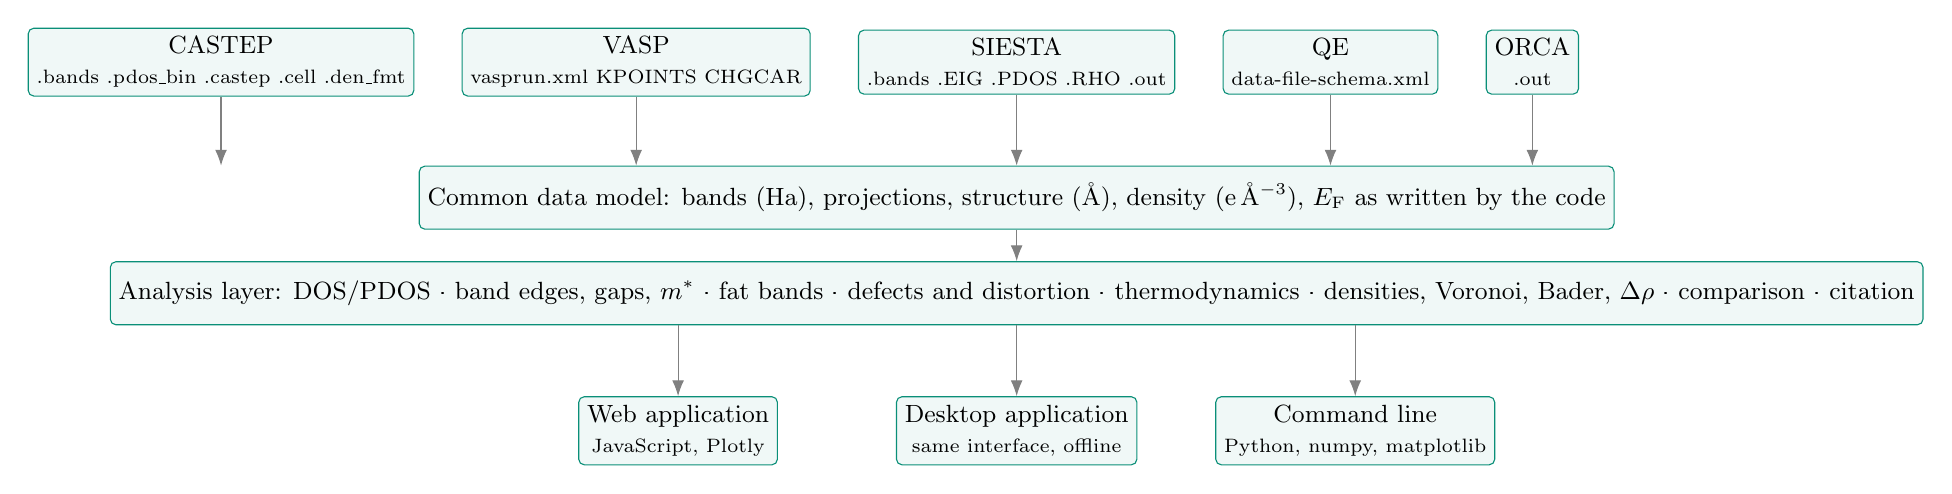
\begin{tikzpicture}[node distance=4mm and 6mm, every node/.style={font=\small},
  box/.style={draw=bmc,rounded corners=2pt,fill=bmc!6,align=center,minimum height=8mm,inner sep=3pt},
  lay/.style={draw=gray!60,rounded corners=4pt,inner sep=5pt}]
\node[box] (c1) {CASTEP\\\scriptsize .bands .pdos\_bin .castep .cell .den\_fmt};
\node[box,right=of c1] (c2) {VASP\\\scriptsize vasprun.xml KPOINTS CHGCAR};
\node[box,right=of c2] (c3) {SIESTA\\\scriptsize .bands .EIG .PDOS .RHO .out};
\node[box,right=of c3] (c4) {QE\\\scriptsize data-file-schema.xml};
\node[box,right=of c4] (c5) {ORCA\\\scriptsize .out};
\node[box,below=9mm of c3,minimum width=13cm] (dm) {Common data model: bands (Ha), projections, structure (\AA), density (e\,\AA$^{-3}$), $E_\mathrm{F}$ as written by the code};
\node[box,below=of dm,minimum width=13cm] (an) {Analysis layer: DOS/PDOS · band edges, gaps, $m^*$ · fat bands · defects and distortion · thermodynamics · densities, Voronoi, Bader, $\Delta\rho$ · comparison · citation};
\node[box,below=9mm of an,xshift=-4.3cm] (f1) {Web application\\\scriptsize JavaScript, Plotly};
\node[box,below=9mm of an] (f2) {Desktop application\\\scriptsize same interface, offline};
\node[box,below=9mm of an,xshift=4.3cm] (f3) {Command line\\\scriptsize Python, numpy, matplotlib};
\foreach \c in {c1,c2,c3,c4,c5} \draw[-{Latex[length=2mm]},gray] (\c.south) -- (dm.north -| \c.south);
\draw[-{Latex[length=2mm]},gray] (dm) -- (an);
\foreach \f in {f1,f2,f3} \draw[-{Latex[length=2mm]},gray] (an.south -| \f.north) -- (\f.north);
\end{tikzpicture}}
\caption{Architecture of \BMR. Code-specific readers convert every output to a common data model; a single set of analyses serves three front-ends with identical semantics.}\label{fig:arch}
\end{figure}

The three front-ends are:
\begin{itemize}
  \item \textbf{Web application.} A single, self-contained HTML document with embedded JavaScript, using Plotly.js for interactive 2D/3D graphics and JSZip for archive export. Files are read locally through the File API; nothing is uploaded. Whole folders can be dropped (needed for VASP, whose files have fixed names).
  \item \textbf{Desktop application.} The same document, with all libraries and fonts bundled, displayed in a native window through pywebview \cite{pywebview} (Microsoft Edge WebView2 on Windows, Qt WebEngine or WebKitGTK on Linux, WebKit on macOS). When no native engine is available it falls back to the default browser, served on the loopback interface only. A Windows installer (Inno Setup) and stand-alone executables (PyInstaller \cite{pyinstaller}) are built by continuous integration.
  \item \textbf{Command line.} A single Python file (\code{brumare.py}, installable with \code{pip install brumare}) depending only on numpy \cite{harris2020numpy} and matplotlib \cite{hunter2007matplotlib}, so that it can be copied to a cluster and run inside batch jobs. It writes PNG/PDF/SVG figures, tab-separated \code{.dat} tables for Origin or gnuplot, VESTA-ready CHGCAR files and text reports.
\end{itemize}

\paragraph{Parity between front-ends.} The JavaScript and Python implementations are written independently but follow the same specification and are cross-checked on the same inputs (Section~\ref{sec:valid}). In Python, non-CASTEP inputs are registered in an in-memory \emph{virtual file registry}: the readers for VASP, SIESTA, QE and ORCA produce objects indexed by the file names the CASTEP pipeline expects (\code{seed.bands}, \code{seed.pdos\_bin}, \ldots), and every CASTEP reader consults the registry before the disk. This design added five codes without modifying the analysis pipeline, and allowed us to verify that the CASTEP results remained byte-identical after each extension.

\section{Input layer}\label{sec:input}
Table~\ref{tab:readers} summarises the readers. Several format details deserve comment because they are frequent sources of silent errors.

\begin{table}[t]\centering\small
\caption{Readers and unit conversions. $1\,\mathrm{Ha}=27.211386245988$\,eV (CODATA 2018), $1\,\mathrm{Bohr}=0.529177$\,\AA.}\label{tab:readers}
\begin{tabularx}{\linewidth}{@{}lXX@{}}\toprule
Code & Files and content & Conversion and remarks \\\midrule
CASTEP & \code{.bands} (Ha, fractional $\bm{k}$), \code{.pdos\_bin} (Fortran unformatted, big-endian), \code{.castep} (Mulliken, energies, forces, valence $Z$), \code{.cell}, \code{.den\_fmt} & \code{.den\_fmt} stores $\rho V$; $\bm{k}$-points of \code{.pdos\_bin} aligned by coordinates \\
VASP & \code{vasprun.xml} (eigenvalues, occupations, PAW projections, structures, energies), \code{KPOINTS} (labels), \code{CHGCAR} & streaming XML parser; CHGCAR stores $\rho V$ \\
SIESTA & \code{.bands} (BandLines/BandPoints), \code{.EIG}+\code{.KP}, \code{.PDOS} (XML curves), \code{.STRUCT\_OUT}/\code{.XV}, \code{.RHO}, \code{.out} & $\rho$ in e\,Bohr$^{-3}$; \code{.KP} in Cartesian Bohr$^{-1}$ \\
QE & \code{data-file-schema.xml} (eigenvalues in Ha, $\bm{k}$ in $2\pi/a$, positions in Bohr, energies) & $\bm{k}_\mathrm{frac}=\bm{k}_\mathrm{cart}\mathbf A^{T}/2\pi$ \\
ORCA & \code{.out} (orbital energies and occupations, final energy, geometry, Mulliken/Löwdin charges) & molecule: one ``$\bm{k}$-point'', box of $\max(\text{extent})+12$\,\AA \\\bottomrule
\end{tabularx}
\end{table}

\paragraph{CASTEP.} The \code{.pdos\_bin} file is a sequence of big-endian Fortran records: a header (number of $\bm{k}$-points, spins, orbitals, maximum number of bands), the species, ion and angular-momentum labels of every orbital, and, for each $\bm{k}$-point and spin, the weight matrix $p^{\alpha}_{n\bm{k} s}$. We found that the $\bm{k}$-index stored in the file may point to the first of several identical $\bm{k}$-points (e.g.\ a repeated $\Gamma$ in a band path); \BMR\ therefore matches the projection $\bm{k}$-points to the band $\bm{k}$-points by their fractional coordinates rather than by index. Pseudopotential shells (e.g.\ Mg 2p and 3p semicore and valence states) and the ordering of the real spherical harmonics are read from the orbital table of the \code{.castep} file.

\paragraph{VASP.} \code{vasprun.xml} files may reach gigabytes; the Python reader uses an event-driven (streaming) XML parser and keeps only the last ionic step. Projections ($s,p_y,p_z,p_x,d_{xy},d_{yz},d_{z^2},d_{xz},d_{x^2-y^2}$, written when \code{LORBIT}$\geq10$) are mapped to the same orbital labels used for CASTEP. For non-collinear runs only the total projection is used. Some VASP versions write a zero $E(\sigma\!\to\!0)$ in the final energy block; in that case the value of the last self-consistent step is used. \code{KPOINTS} files in line mode provide the vertex labels, including path discontinuities (e.g.\ K$|$U).

\paragraph{SIESTA.} Two \code{.bands} formats exist: \emph{BandLines} (cumulative path length and vertex labels) and \emph{BandPoints} (Cartesian $\bm{k}$-points without labels); both are recognised. When both \code{.bands} and \code{.EIG} are present, bands are taken from the path and the DOS from the self-consistent mesh. The \code{.PDOS} file already contains broadened projected curves per orbital $(n,l,m,\zeta)$; these are interpolated on the energy grid instead of being recomputed, and projected bands are consequently unavailable. The binary \code{.RHO} is read record by record.

\paragraph{Quantum ESPRESSO and ORCA.} The QE reader extracts eigenvalues, occupations, $\bm{k}$-points and weights, the Fermi energy (or the highest occupied level), the cell and positions from the XML schema. The ORCA reader extracts the last orbital-energy block (restricted or unrestricted), the final single-point energy, the Cartesian geometry and Mulliken and Löwdin charges; for molecules the band diagram becomes an energy-level diagram and the gap is the HOMO–LUMO gap.

\section{Methods}\label{sec:methods}
\subsection{Energy reference and the Fermi level}
Let $\eF^{s}$ be the Fermi energy written by the code for spin $s$. \BMR\ never recomputes it. Energies are displayed either in the \emph{original} scale (default), with a dash-dotted line at $\eF$ and its value printed on every panel, or shifted,
\begin{equation}
\tilde\varepsilon_{n\bm{k} s}=\varepsilon_{n\bm{k} s}-E_\mathrm{ref}^{s},\qquad E_\mathrm{ref}^{s}\in\Big\{\eF^{s},\ \eF^{\uparrow},\ \eF^{\downarrow},\ \tfrac12(\eF^{\uparrow}+\eF^{\downarrow}),\ 0\Big\}.
\end{equation}
The plotting window $[E_\mathrm{min},E_\mathrm{max}]$ is always defined relative to $\eF$, so that in the original scale the axis spans $[\bar E_\mathrm{F}+E_\mathrm{min},\bar E_\mathrm{F}+E_\mathrm{max}]$ for any material. Because absolute eigenvalues of different calculations (and, a fortiori, of different codes) refer to different potential references, multi-calculation comparisons always align each calculation to its own $\eF$.

\subsection{Band path and high-symmetry labels}
With direct lattice vectors as rows of $\mathbf A$ (Bohr), the reciprocal lattice is $\mathbf B=2\pi(\mathbf A^{-1})^{T}$ and the Cartesian $\bm{k}$-vector is $\bm{k}_\mathrm{cart}=\bm{k}_\mathrm{frac}\mathbf B$. The abscissa of the band plot is the cumulative path length
\begin{equation}
x_i=\sum_{j=1}^{i}\lVert(\bm{k}_j-\bm{k}_{j-1})\mathbf B\rVert ,
\end{equation}
where steps larger than a threshold are treated as discontinuities (zero length, composite label). Vertices are detected where the direction of $\bm{k}_j-\bm{k}_{j-1}$ changes or a repeated point occurs, and are labelled by matching their fractional coordinates to the high-symmetry points of the detected Bravais lattice \cite{setyawan2010}; user labels override the detection.

\subsection{Density of states and projections}
The total and projected densities of states are Gaussian-broadened sums over bands and $\bm{k}$-points,
\begin{gather}
g_s(E)=\sum_{\bm{k}}w_{\bm{k}}\sum_n\delta_\sigma(E-\varepsilon_{n\bm{k} s}),\qquad
\delta_\sigma(x)=\frac{e^{-x^2/2\sigma^2}}{\sigma\sqrt{2\pi}},\\
g^{G}_s(E)=\sum_{\bm{k}}w_{\bm{k}}\sum_n\Big(\sum_{\alpha\in G}p^{\alpha}_{n\bm{k} s}\Big)\delta_\sigma(E-\varepsilon_{n\bm{k} s}),
\end{gather}
with normalised weights $\sum_{\bm{k}}w_{\bm{k}}=1$. A group $G$ is a set of orbitals defined at one of five levels: element, angular momentum $l$, pseudopotential shell $(n,l)$, magnetic component $m$ (real harmonics), or individual atoms; for $d$ orbitals the octahedral $t_{2g}=\{d_{xy},d_{yz},d_{xz}\}$ and $e_g=\{d_{z^2},d_{x^2-y^2}\}$ sums are provided (in the Cartesian axes of the cell). For spin-polarised systems the spin-down DOS is optionally plotted with negative sign. Integrated occupations and the $d$-band centre \cite{hammer1995} are
\begin{equation}
N^{G}_s=\int_{-\infty}^{\eF}g^{G}_s(E)\,dE,\qquad \varepsilon_d=\frac{\int E\,g^{d}(E)\,dE}{\int g^{d}(E)\,dE},
\end{equation}
the latter evaluated up to $\eF$ (occupied) and over the whole window. The spin polarisation at the Fermi level,
\begin{equation}
P=\frac{N_\uparrow(\eF)-N_\downarrow(\eF)}{N_\uparrow(\eF)+N_\downarrow(\eF)},
\end{equation}
is reported only when $N_\uparrow+N_\downarrow>0.05$ states/eV; otherwise $\eF$ lies in a gap and the ratio is undefined. When a code supplies broadened curves (SIESTA), $g^{G}_s$ is obtained by linear interpolation of the summed curves.

\subsection{Band edges, gaps and effective masses}
For $N_s$ electrons in spin channel $s$ (half of the total for spin-degenerate runs), the highest occupied and lowest unoccupied bands are $N_s$ and $N_s+1$:
\begin{equation}
E_\mathrm{VBM}^{s}=\max_{\bm{k}}\varepsilon_{N_s,\bm{k} s},\qquad E_\mathrm{CBM}^{s}=\min_{\bm{k}}\varepsilon_{N_s+1,\bm{k} s},\qquad E_g^{s}=E_\mathrm{CBM}^{s}-E_\mathrm{VBM}^{s},
\end{equation}
and the total gap of a spin-polarised system is $\min_s E_\mathrm{CBM}^{s}-\max_s E_\mathrm{VBM}^{s}$. The gap is direct when both extrema occur at the same $\bm{k}$. If $\eF$ lies inside a band within 5\,meV, the channel is flagged as metallic or partially occupied; for fractional occupations (smearing) the electron count is taken from the occupations. Effective masses are obtained by parabolic fits around the extremum along the path,
\begin{equation}
E(k)\simeq c_0+c_1(k-k_0)+c_2(k-k_0)^2,\qquad \frac{m^*}{m_e}=\pm\frac{\hbar^2}{2m_e\,c_2},\qquad \frac{\hbar^2}{m_e}=7.619964\ \mathrm{eV\,\text{\AA}^2},
\end{equation}
with the positive (negative) sign for electrons (holes). If the extremum lies inside a segment, a five-point fit with a linear term locates the true minimum between $\bm{k}$-points; if it lies at a vertex (e.g.\ $\Gamma$), one mass is reported for each direction using $E=a(k-k_0)^2+c$. Masses are computed only for continuous paths and when $\eF$ is in the gap.


\subsection{Band-gap correction}\label{sec:gapcorr}
Semilocal functionals (LDA, GGA) systematically underestimate band gaps, typically by 30–100\%. The origin is not a numerical deficiency of any particular code but the interpretation of Kohn–Sham eigenvalues as quasiparticle energies: the Kohn–Sham gap lacks the derivative discontinuity $\Delta_\mathrm{xc}$ of the exchange-correlation potential \cite{perdew1983,sham1983}, so that $E_g=E_g^\mathrm{KS}+\Delta_\mathrm{xc}$, and semilocal approximations additionally suffer from delocalisation error \cite{morisanchez2008}. A proper treatment requires hybrid functionals such as HSE06 \cite{heyd2003}, meta-GGAs, DFT+U or many-body ($GW$) corrections, which must be applied in the electronic-structure calculation itself. As a post-processing alternative, \BMR\ implements the \emph{scissor} correction \cite{levine1989}, a rigid upward shift of the unoccupied bands,
\begin{equation}
\varepsilon^\mathrm{corr}_{n\bm{k} s}=\varepsilon_{n\bm{k} s}+\Delta\,\Theta(n-N_s-\tfrac12),\qquad E_g^\mathrm{corr}=E_g^\mathrm{DFT}+\Delta,
\end{equation}
where $\Theta$ is the Heaviside step and $N_s$ the number of occupied bands in channel $s$; occupied bands and the Fermi energy written by the code are left untouched. Three choices of $\Delta$ are offered: (i) a user-supplied value; (ii) a reference gap $E_g^\mathrm{ref}$ (experimental, hybrid or $GW$), $\Delta=E_g^\mathrm{ref}-E_g^\mathrm{DFT}$; and (iii) the empirical linear model of Morales-García, Valero and Illas \cite{morales2017}, obtained from 66 semiconductors and insulators with experimental gaps between 0.1 and 9\,eV,
\begin{equation}
E_g^{G_0W_0}=1.358\,E_g^\mathrm{PBE}+0.904\ \mathrm{eV}\quad(r=0.91),\qquad E_g^\mathrm{exp}=0.998\,E_g^{G_0W_0}+0.014\ \mathrm{eV},
\end{equation}
which gives $\Delta=0.358\,E_g^\mathrm{PBE}+0.904$\,eV. The model was fitted to PBE gaps and is not used for LDA, metals or vanishing PBE gaps; the authors excluded six strongly correlated transition-metal oxides (MnO, ZnO, CoO, SnO$_2$, CuAlO$_2$, CuInO$_2$) that deviate by about 2\,eV, and report mean absolute errors of 0.23\,eV ($G_0W_0$ versus experiment) for non-oxides. Because a scissor is a rigid shift, it leaves band dispersions and effective masses unchanged and cannot correct the position of empty defect levels within the gap; in defective supercells, $\Delta$ is best determined from the pure host. All three options are available in every front-end, the original DFT gap is always reported next to the corrected one, and the model reference is added to the session's BibTeX file when used.


\subsection{Brillouin zone and band paths}\label{sec:bz}
The first Brillouin zone is constructed as the Wigner--Seitz cell of the reciprocal lattice, $\mathrm{BZ}=\{\bm k:\ \bm k\cdot\mathbf G\le\tfrac12|\mathbf G|^2\ \forall\,\mathbf G\neq0\}$. The reciprocal basis $\mathbf b_i=2\pi(\mathbf a_j\times\mathbf a_k)/V$ is first reduced with the LLL algorithm \cite{lenstra1982}; the Bragg planes of the 26 shortest $\mathbf G$ vectors are intersected three at a time, the intersections that satisfy every inequality become vertices, the vertices lying on each plane form a face, and the geometric volume $\sum_f\tfrac13A_f|\mathbf G_f|/2$ is checked against $V_\mathrm{BZ}=(2\pi)^3/V$ (the search is enlarged to $|n_i|\le2$ otherwise). The lattice type is recognised from the shape of the zone (cube, square or rectangular prism, truncated octahedron, rhombic dodecahedron or hexagonal prism) after an optional symmetry tolerance (0.5$^\circ$ and 0.5\% by default) that idealises slightly distorted relaxed cells. High-symmetry points are face centres $\mathbf G/2$, edge midpoints and vertices, labelled following Setyawan and Curtarolo \cite{setyawan2010}; consecutive points of the standard path are taken as the nearest equivalent copies, so that every segment follows a symmetry line. Fractional coordinates $k_i=\mathbf a_i\cdot\bm k/2\pi$ refer to the cell used in the calculation, and ready-to-use inputs are written for CASTEP (\code{SPECTRAL\_KPOINT\_PATH}), VASP (line-mode \code{KPOINTS}), Quantum ESPRESSO (\code{K\_POINTS crystal\_b}) and SIESTA (\code{BandLines}), together with Monkhorst--Pack meshes $n_i=\lceil|\mathbf b_i|/\Delta k\rceil$. When only the lattice is known, low-symmetry lattices receive an automatic path through the face centres, and SeeK-path \cite{hinuma2017} provides the alternative crystallographic convention. When atoms are available, the space group is first determined with moyo \cite{moyo}, the successor of spglib \cite{togo2024spglib} (the same library family used by SeeK-path), through identical Python and WebAssembly builds; the zone is then built on the standardized primitive cell, which is exported together with the conventional cell, and all 14 Bravais lattices (the 25 cases of Setyawan--Curtarolo, from CUB to TRI) receive their standard points and paths, defined in the primitive basis of the original paper, mapped onto the standardized basis by an integer unimodular transformation and accepted only if every point lies on the zone surface; for triclinic lattices the reduced reciprocal basis with all-acute or all-obtuse angles of minimal norm is used. Structures are read from CIF (with expansion of the symmetry operations), POSCAR, CASTEP \code{.cell}, XSF, Quantum ESPRESSO input and extended XYZ files, from the Crystallography Open Database, or from a built-in library of 51 materials with literature lattice parameters.

\subsection{Projected (fat) bands}
In projected-band plots the marker size is $s_{n\bm{k}}=s_\mathrm{max}\sum_{\alpha\in G}p^{\alpha}_{n\bm{k} s}$, drawn on top of the plain band structure, with one panel per group or overlaid groups.

\subsection{Structure, point defects and distortion}
Interatomic vectors use the minimum-image convention, $\Delta\mathbf f=\mathbf f_j-\mathbf f_i-\operatorname{round}(\mathbf f_j-\mathbf f_i)$ and $d_{ij}=\lVert\Delta\mathbf f\,\mathbf A\rVert$. \emph{With a pure reference structure}, every defective-cell atom is matched to the nearest reference site of the same or a different species; unmatched reference sites are vacancies, sites occupied by another species are substitutions and unmatched defect atoms are interstitials. \emph{Without a reference}, the defect is located by species rarity and coordination anomalies, and local quantities are compared with the "bulk" of the same supercell (atoms farther than a cutoff from the defect). The first coordination shell contains the neighbours with $d<f\,d_\mathrm{min}$ ($f=1.25$ by default). For a polyhedron with $n$ ligands at distances $d_i$, mean $\bar d$, and $m$ ligand–centre–ligand angles $\theta_j$, \BMR\ reports Baur's distortion index \cite{baur1974}, the quadratic elongation and angle variance of Robinson, Gibbs and Ribbe \cite{robinson1971}, and Hoppe's effective coordination number \cite{hoppe1979}:
\begin{gather}
D=\frac1n\sum_{i=1}^{n}\frac{|d_i-\bar d|}{\bar d},\qquad
\langle\lambda\rangle=\frac1n\sum_{i=1}^{n}\Big(\frac{d_i}{l_0}\Big)^2,\qquad
\sigma^2=\frac{1}{m-1}\sum_{j=1}^{m}(\theta_j-\theta_0)^2,\\
\mathrm{ECoN}=\sum_{i}\exp\!\Big[1-\Big(\frac{d_i}{d_\mathrm{av}}\Big)^6\Big],\qquad
d_\mathrm{av}=\frac{\sum_i d_i\exp[1-(d_i/d_\mathrm{min})^6]}{\sum_i\exp[1-(d_i/d_\mathrm{min})^6]},
\end{gather}
where $l_0$ is the centre-to-vertex distance of the regular polyhedron of the same volume and $\theta_0=90^\circ$ (octahedron) or $109.47^\circ$ (tetrahedron). The polyhedron volume is that of the convex hull of the ligands. With a reference, the displacement field $\mathbf u_i=\Delta\mathbf f_i\mathbf A$ is reported as a function of the distance to the defect, together with the perturbation radius beyond which $|\mathbf u_i|$ falls below a threshold, and the relative cell-volume change $\Delta V/V$.

\subsection{Defect and hydride thermodynamics}
With chemical potentials $\mu_i$ given by the energy per atom of elemental references computed with the same parameters (e.g.\ hcp Mg, bcc Fe and $\mu_\mathrm{H}=\tfrac12E(\mathrm H_2)$), the defect formation energy \cite{freysoldt2014,vandewalle2004}, the hydride formation enthalpy per mole of H$_2$, the defect effect and the desorption temperature are
\begin{gather}
E_f=E_\mathrm{def}-E_\mathrm{pure}-\sum_i n_i\mu_i,\qquad
\Delta H_f=\frac{E-\sum_iN_i\mu_i}{N_\mathrm H/2},\qquad
\Delta\Delta H=\Delta H_f^\mathrm{def}-\Delta H_f^\mathrm{pure},\\
T_d=\frac{\Delta H_f}{\Delta S},\qquad \Delta S\simeq S^\circ(\mathrm H_2,\mathrm g)=130.7\ \mathrm{J\,mol^{-1}K^{-1}},
\end{gather}
with $n_i>0$ for added atoms and $\Delta S$ taken from JANAF \cite{chase1998janaf}. The hydrogen-removal energy is $E_\mathrm{rem}=E(\text{H-deficient})+\mu_\mathrm H-E$, and the gravimetric and volumetric capacities are $w_\mathrm H=N_\mathrm H m_\mathrm H/\sum_iN_im_i$ and $\rho_\mathrm H=N_\mathrm H m_\mathrm H/V$. For metals the total energy is extrapolated to zero smearing ($E-\tfrac12TS$); the energy type is selectable. These are electronic energies at 0\,K without zero-point or vibrational contributions, so $T_d$ is an estimate suitable for comparing trends.

\subsection{Charge densities}
CASTEP (\code{.den\_fmt}) and VASP (\code{CHGCAR}) store $\rho V$; Gaussian cube files and the SIESTA binary density (\code{.RHO}) store $\rho$ in e\,Bohr$^{-3}$. All are converted to $\rho$ in e\,\AA$^{-3}$ and checked through $\int\rho\,dV=(V/N)\sum_{\mathbf r}\rho(\mathbf r)=N_e$. Spin densities $\rho_\uparrow-\rho_\downarrow$, $|\rho_\uparrow-\rho_\downarrow|$ and $\zeta=(\rho_\uparrow-\rho_\downarrow)/\rho$ are derived when both channels are present. Off-grid values are obtained by periodic trilinear interpolation,
\begin{equation}
\rho(\mathbf f)=\sum_{a,b,c\in\{0,1\}}\rho_{i+a,j+b,k+c}\,\big[(1-t_1)^{1-a}t_1^{a}\big]\big[(1-t_2)^{1-b}t_2^{b}\big]\big[(1-t_3)^{1-c}t_3^{c}\big],
\end{equation}
with $t_\nu$ the fractional offsets inside the grid cell. Isosurfaces use marching cubes \cite{lorensen1987} on a Cartesian resampling. Two-dimensional slices are defined by three atoms or by Miller indices $(hkl)$; the multiplicity of the supercell with respect to the primitive (base) cell is detected, so that indices refer to the material (e.g.\ rutile MgH$_2$) rather than to the supercell, and the interplanar spacing is $d_{hkl}=2\pi/\lVert(h,k,l)\,\mathbf B_\mathrm{base}\rVert$. A gallery shows several planes through the defect, a slider shifts the plane along its normal, and line profiles along bonds report the density minimum as an approximation to the bond critical point of the quantum theory of atoms in molecules \cite{bader1990}.

\subsection{Atomic charges and moments}
Three partitions are provided. Mulliken populations \cite{mulliken1955,segall1996} are read from CASTEP and ORCA. In the \emph{Voronoi} partition \cite{voronoi1908} each grid point belongs to the nearest atom, or, in the radical (power) variant \cite{gellatly1982}, to the atom minimising $\lVert\mathbf r-\mathbf R_a\rVert^2-r_a^2$ with covalent radii $r_a$ \cite{cordero2008}:
\begin{equation}
N_a=\int_{V_a}\rho\,dV,\qquad q_a=Z_a^\mathrm{val}-N_a,\qquad m_a=\int_{V_a}(\rho_\uparrow-\rho_\downarrow)\,dV .
\end{equation}
In the \emph{Bader} partition \cite{bader1990}, the on-grid algorithm of Henkelman, Arnaldsson and Jónsson \cite{henkelman2006} assigns to each grid point the neighbour (among 26) of steepest ascent, $\arg\max_{\mathbf r'}[\rho(\mathbf r')-\rho(\mathbf r)]/\lVert\mathbf r'-\mathbf r\rVert$. Following these pointers leads to density maxima; \BMR\ resolves the chains by pointer jumping (repeated composition $t\leftarrow t\circ t$, converging in $O(\log L)$ vectorised passes for chains of length $L$), and assigns each maximum (basin) to the nearest atom. Boundary points are then reassigned with the near-grid method of Tang et al.\ \cite{tang2009bader}, which follows the true density gradient with a correction vector that accumulates the difference between the ideal and the on-grid step and so removes the lattice bias; the trajectories of all boundary points are advanced simultaneously, and the procedure is repeated until the boundaries no longer change. The browser application uses the on-grid assignment alone, which is faster and adequate for interactive exploration.

\subsection{Density difference and charge redistribution}
For a defective density $\rho_A$ and references $\rho_B$ (pure host, preferably in the defect geometry) and optionally $\rho_C$ (isolated dopant), the difference $\Delta\rho=\pm(\rho_A-\rho_B-\rho_C)$ is evaluated on the grid of $\rho_A$ (references are resampled trilinearly when grids differ). \BMR\ reports
\begin{gather}
Q_\pm=\int_{\Delta\rho\gtrless0}\Delta\rho\,dV,\qquad \Delta N=Q_++Q_-,\qquad Q_\mathrm{red}=\tfrac12\int|\Delta\rho|\,dV,\\
\mathbf p=\int(\mathbf r-\mathbf r_c)\,\Delta\rho\,dV\ \ [1\ e\,\text{\AA}=4.80320\ \mathrm D],\qquad
\Delta Q(r)=\int_0^{r}\overline{\Delta\rho}(r')\,4\pi r'^2\,dr',
\end{gather}
where $\overline{\Delta\rho}(r)$ is the spherical average around the defect centre $\mathbf r_c$ (minimum-image distances), and the radii $R_{50}$ and $R_{90}$ that enclose 50\% and 90\% of $\int|\Delta\rho|dV$. The dipole depends on the origin when $\Delta N\neq0$, which is reported. Planar averages along each lattice vector, the per-atom charge transfer in Voronoi cells and the density minimum of every dopant–ligand bond compared with the same host bond in the pure structure complete the analysis.

\subsection{Comparison of calculations and citation tracking}
Any number of calculations (from any code) can be compared in a table with one column per calculation (energies, $E_f$, $\Delta H$, $\Delta\Delta H$, $T_d$, $\eF$, gaps and their type, $N(\eF)$, polarisation, $d$ occupation and moment, charges, density at the bond minimum, coordination, bond lengths, distortion indices, displacements, $\Delta V/V$, cell parameters and residual force), exported as \code{.dat}, and in plots of overlaid DOS and PDOS (aligned at each $\eF$), side-by-side band structures, bar charts and density slices on a common plane. Mesh calculations without a band path are excluded from band panels. During a session, \BMR\ records which analyses were used and generates a BibTeX file containing the software itself, the electronic-structure codes whose outputs were loaded and the method references actually invoked (e.g.\ Setyawan–Curtarolo paths \cite{setyawan2010}, Voronoi or Bader partitions, Robinson distortion indices, Mulliken analysis, VESTA export).

\section{Implementation}\label{sec:impl}
The web application is a single HTML file of about 4500 lines with 241 JavaScript functions; the command-line program is a single Python file of about 4000 lines with 95 functions. Plotly.js 2.27 renders all interactive figures, including 3D isosurfaces; a plot editor stores per-curve colours, names, line styles and visibility across tabs. Figures are exported at publication resolution as PNG, JPEG, WebP, SVG or JPEG~XL, individually or all at once in a ZIP archive; JPEG~XL is encoded in the browser by the reference libjxl compiled to WebAssembly (lossless mode verified to be pixel-identical to PNG at about two thirds of its size) and on the command line through imagecodecs, where \code{--format png,jxl,svg,pdf} writes every figure in all requested formats. Other exports include tab-separated tables with a header line (recognised by Origin as long names), CHGCAR files in VASP~5 format with element names (as $\rho V$, readable by VESTA and \code{bader}), XSF files and ZIP archives with one folder per structure.

\paragraph{Internationalisation.} The interface, help and tutorial are available in six languages (Portuguese, English, Spanish, French, Italian and Latin). A small engine translates rendered text nodes and attributes through a dictionary of about 730 entries plus regular-expression rules for strings containing numbers (e.g.\ ``1.3942 indirect''); it stores the original text of each node, observes the document with a \code{MutationObserver} so that content produced later by the analyses is also translated, and ignores elements marked \code{translate="no"}. Numerical results are never altered. Long documents (the tutorial) have one page per language, generated from translated bodies, with \code{hreflang} metadata, and PDF versions are produced from the same pages with pandoc and XeLaTeX.

\paragraph{Packaging and distribution.} The Python package (\code{pip install brumare}) provides the commands \code{brumare} (command line), \code{brumare-gui} (desktop application) and \code{brumare-lote} (batch analysis with a minimal window). Continuous integration builds the Windows executables and installer for every tagged release and publishes the package to PyPI through trusted publishing. The software is released under the GPL-3.0-or-later \cite{gplv3}; bundled third-party components (Plotly.js and JSZip under MIT, MathJax under Apache~2.0, fonts under the SIL Open Font License) are compatible with it.

\paragraph{Testing.} An automated test suite (80 \code{pytest} tests on real outputs of the five codes, covering band gaps, effective masses, magnetic moments, the band-gap correction, lossless JPEG~XL export, Bader charge conservation, citation output and the translated command-line help, plus the cross-validation of Table~\ref{tab:bench}) runs under continuous integration on Python 3.9 and 3.12.

\section{Validation}\label{sec:valid}
\paragraph{Internal consistency.} The integrated density reproduces the number of valence electrons (e.g.\ $\int\rho\,dV=40.000$ for SrTiO$_3$ from SIESTA). A \code{.den\_fmt}$\to$CHGCAR$\to$read round trip changes the density by $\sim10^{-8}$, and the CHGCAR files written by the JavaScript and Python implementations differ by $\sim10^{-6}$ (relative), at the level of the printed precision. After each extension of the input layer, all CASTEP outputs of a reference calculation were compared byte by byte with those of the previous version. The density-difference report, the comparison table and the effective masses give the same numbers in the browser and on the command line.

\paragraph{Reference systems.} Table~\ref{tab:valid} lists results obtained with real output files distributed with the test suites of pymatgen (VASP), sisl (SIESTA), Quantum ESPRESSO and cclib (ORCA). The PBE band gap of Si (0.614\,eV, indirect from $\Gamma$ to near X) and the longitudinal electron mass ($m^*_l=0.94\,m_e$, experiment $0.92\,m_e$) agree with the literature for this functional; the ferromagnetic Fe$_2$O$_3$ cell computed with LDA+U carries 20\,$\mu_\mathrm B$ (56 spin-up and 36 spin-down electrons), as expected for four high-spin Fe$^{3+}$ ions; the SrTiO$_3$ LDA calculation shows an indirect R$\to\Gamma$ gap of 2.25\,eV with O~2p valence and crystal-field-split Ti~3d $t_{2g}/e_g$ conduction states, and the integrated density matches the 40 valence electrons. In every case the analysis reproduces the physical picture expected for these well-studied systems. The band-gap correction illustrates the limits of empirical models: for Si the PBE$\to G_0W_0$ relation predicts 1.738\,eV against the experimental 1.17\,eV, an error within the scatter of the original fit but large in absolute terms for small-gap semiconductors; the scissor to the experimental value restores 1.170\,eV exactly, with identical effective masses, as expected for a rigid shift. The browser and command-line implementations give identical corrected gaps.

\begin{table}[t]\centering\small
\caption{Validation with real outputs. Gaps are Kohn–Sham gaps of the functional used in each calculation.}\label{tab:valid}
\begin{tabularx}{\linewidth}{@{}llX@{}}\toprule
Code & System & \BMR\ result \\\midrule
CASTEP & MgH$_2$:Fe (162-atom supercell, spin) & $\eF=1.837$\,eV; total gap 1.394\,eV, indirect M$\to$R; Fe–H 1.649–1.653\,\AA \\
VASP & Si, line-mode bands (PBE) & gap 0.614\,eV indirect; $m^*_e=0.94\,m_e$; $m^*_h(\Gamma)=0.32\,m_e$ \\
VASP & Si, gap correction (Section~\ref{sec:gapcorr}) & empirical model 1.738\,eV; scissor to experiment 1.170\,eV; masses unchanged \\
VASP & Fe$_2$O$_3$, ferromagnetic (LDA+U) & 56$\uparrow$/36$\downarrow$ electrons, 20\,$\mu_\mathrm B$; $P(\eF)$ undefined ($\eF$ in gap) \\
SIESTA & SrTiO$_3$, spin-polarised (LDA) & gap 2.25\,eV indirect R$\to\Gamma$; $t_{2g}$ below $e_g$; $\int\rho\,dV=40.000$\,e \\
SIESTA & Bi$_2$Se$_3$ (no spin--orbit) & gap 0.042\,eV, direct; eigenvalues identical to sisl \\
QE & Si, test-suite reference (2 $\bm{k}$-points) & gap 1.32\,eV on the coarse mesh \\
ORCA & divinylbenzene (molecule) & HOMO–LUMO gap 5.18\,eV; Mulliken and Löwdin charges \\\bottomrule
\end{tabularx}
\end{table}

\paragraph{Cross-validation against established tools.} Table~\ref{tab:bench} compares \BMR\ with pymatgen, sumo, sisl, cclib and pybader on the same output files (script \code{tools/comparar\_ferramentas.py}). Gaps, band edges, Fermi energies, spin-resolved electron counts and molecular-orbital energies agree to the printed precision ($|\Delta|\le10^{-4}$\,eV). Two differences are methodological and favour the approach adopted here. (i) For MgH$_2$:Fe, the highest occupied band exceeds the Fermi energy written by CASTEP by only 0.04--0.17\,meV (an offset far below any physical energy scale, presumably because the Fermi level is determined on the self-consistent mesh rather than on the band-path $\bm k$-points); tools based on pymatgen therefore classify the system as metallic and report a zero gap, whereas electron counting yields 1.394\,eV, identical (to $10^{-4}$\,eV) to the value obtained by applying the same criterion to the eigenvalues parsed by sumo. (ii) For Si, the conduction-band minimum lies between two $\mathbf{k}$-points of the path; a parabola anchored at the sampled $\mathbf{k}$-point yields one-sided masses of 0.68 and 1.54\,$m_e$ (sumo), whereas the fit with a linear term used by \BMR\ locates the true minimum and gives 0.94\,$m_e$, close to the experimental 0.92\,$m_e$. For the 162-atom MgH$_2$:Fe density, the refined Bader charges agree with pybader within $8\times10^{-4}$\,e per atom on average (0.026\,e at most), with identical total charge, compared with 0.013\,e for the on-grid assignment alone; the refined partition took 0.7\,s, against 1.2\,s for pybader. The Brillouin zones of the six recognised lattice types reproduce $V_\mathrm{BZ}=(2\pi)^3/V$ to $10^{-6}$ and, for FCC Si, the exact distances $|X|=2\pi/a$, $|L|=\sqrt3\pi/a$, $|W|=\sqrt5\pi/a$ and $|K|=3\sqrt2\pi/2a$. The space groups of all 51 library materials and of seven reference structures read from symmetrised CIF and POSCAR files are recovered in both implementations, with identical high-symmetry points in the browser and on the command line; for the MgH$_2$:Fe supercell, moyo finds the base-centred orthorhombic group $Cmmm$ produced by the defect and the relaxation, and the corresponding ORCC path is used. For 18 reference structures covering all 14 Bravais lattices and 23 of the 25 Setyawan--Curtarolo cases (the remaining MCLC4 is a measure-zero boundary case), every high-symmetry point lies on the zone surface, the moduli $|\bm k|$ agree with the independent implementation in pymatgen \cite{ong2013pymatgen} to $10^{-8}$\,\AA$^{-1}$ (triclinic lattices, whose reduced basis is not unique, and the boundary case ORCF3 excepted), and the browser and Python give identical points. This check also exposed that the point $F_3$ listed for MCLC1 in the original paper does not lie on the zone surface; it is not part of the path and is omitted, as in pymatgen.
\begin{table}[t]\centering\small
\caption{Cross-validation of \BMR\ against established tools on the same output files. $|\Delta|$ is the absolute difference.}\label{tab:bench}
\resizebox{\linewidth}{!}{\begin{tabular}{@{}lllrrlr@{}}\toprule
Code & System & Quantity & \BMR & Reference & Tool & $|\Delta|$ \\\midrule
VASP & Si (PBE) & gap (eV) & 0.6143 & 0.6143 & pymatgen & 1.1e-16 \\
VASP & Si (PBE) & $E_\mathrm{F}$ (eV) & 5.8561 & 5.8561 & pymatgen & 1.3e-05 \\
VASP & Si (PBE) & CBM$-$VBM (eV) & 0.6143 & 0.6143 & pymatgen & 1.1e-16 \\
VASP & Si (PBE) & $m^*_e$, side 1 ($m_e$) & 0.9410 & 0.6771 & sumo & 2.6e-01 \\
VASP & Si (PBE) & $m^*_e$, side 2 ($m_e$) & 0.9410 & 1.5400 & sumo & 6.0e-01 \\
VASP & Si (PBE) & $m^*_e$ vs experiment ($m_e$) & 0.9410 & 0.9200 & experiment & 2.1e-02 \\
VASP & Fe$_2$O$_3$ (LDA+U) & moment ($\mu_\mathrm{B}$) & 20.0000 & 20.0000 & pymatgen & 1.6e-06 \\
VASP & Fe$_2$O$_3$ (LDA+U) & gap $\uparrow$ (eV) & 4.0199 & 4.0199 & pymatgen & 0.0e+00 \\
VASP & Fe$_2$O$_3$ (LDA+U) & gap $\downarrow$ (eV) & 2.1923 & 2.1923 & pymatgen & 0.0e+00 \\
CASTEP & MgH$_2$:Fe (162 at.) & total gap (eV) & 1.3940 & 0.0000 & sumo & 1.4e+00 \\
CASTEP & MgH$_2$:Fe (162 at.) & $E_\mathrm{F}$ (eV) & 1.8368 & 1.8368 & sumo & 4.2e-06 \\
CASTEP & MgH$_2$:Fe (162 at.) & gap, electron counting on sumo eigenvalues (eV) & 1.3940 & 1.3941 & sumo & 7.4e-05 \\
SIESTA & SrTiO$_3$ (LDA) & total gap (eV) & 2.2500 & 2.2500 & sisl & 0.0e+00 \\
SIESTA & Bi$_2$Se$_3$ & gap (eV) & 0.0418 & 0.0418 & sisl & 6.0e-16 \\
ORCA & divinylbenzene & HOMO (eV) & -4.0652 & -4.0652 & cclib & 1.8e-05 \\
ORCA & divinylbenzene & LUMO (eV) & 1.1197 & 1.1197 & cclib & 5.9e-06 \\
ORCA & divinylbenzene & HOMO--LUMO gap (eV) & 5.1849 & 5.1849 & cclib & 1.2e-05 \\
CHGCAR & MgH$_2$:Fe CHGCAR (162 at.) & Bader (on-grid) mean $|\Delta q|$ (e) & 0.0000 & 0.0127 & pybader & 1.3e-02 \\
CHGCAR & MgH$_2$:Fe CHGCAR (162 at.) & Bader (refined) mean $|\Delta q|$ (e) & 0.0000 & 0.0008 & pybader & 8.0e-04 \\
CHGCAR & MgH$_2$:Fe CHGCAR (162 at.) & Bader $\sum q$ (e) & 651.0000 & 651.0000 & pybader & 2.3e-13 \\
CHGCAR & MgH$_2$:Fe CHGCAR (162 at.) & Bader (refined) max.\ $|\Delta q|$ (e) & 0.0000 & 0.0257 & pybader & 2.6e-02 \\
\bottomrule\end{tabular}}
\end{table}


\begin{figure}[t]\centering
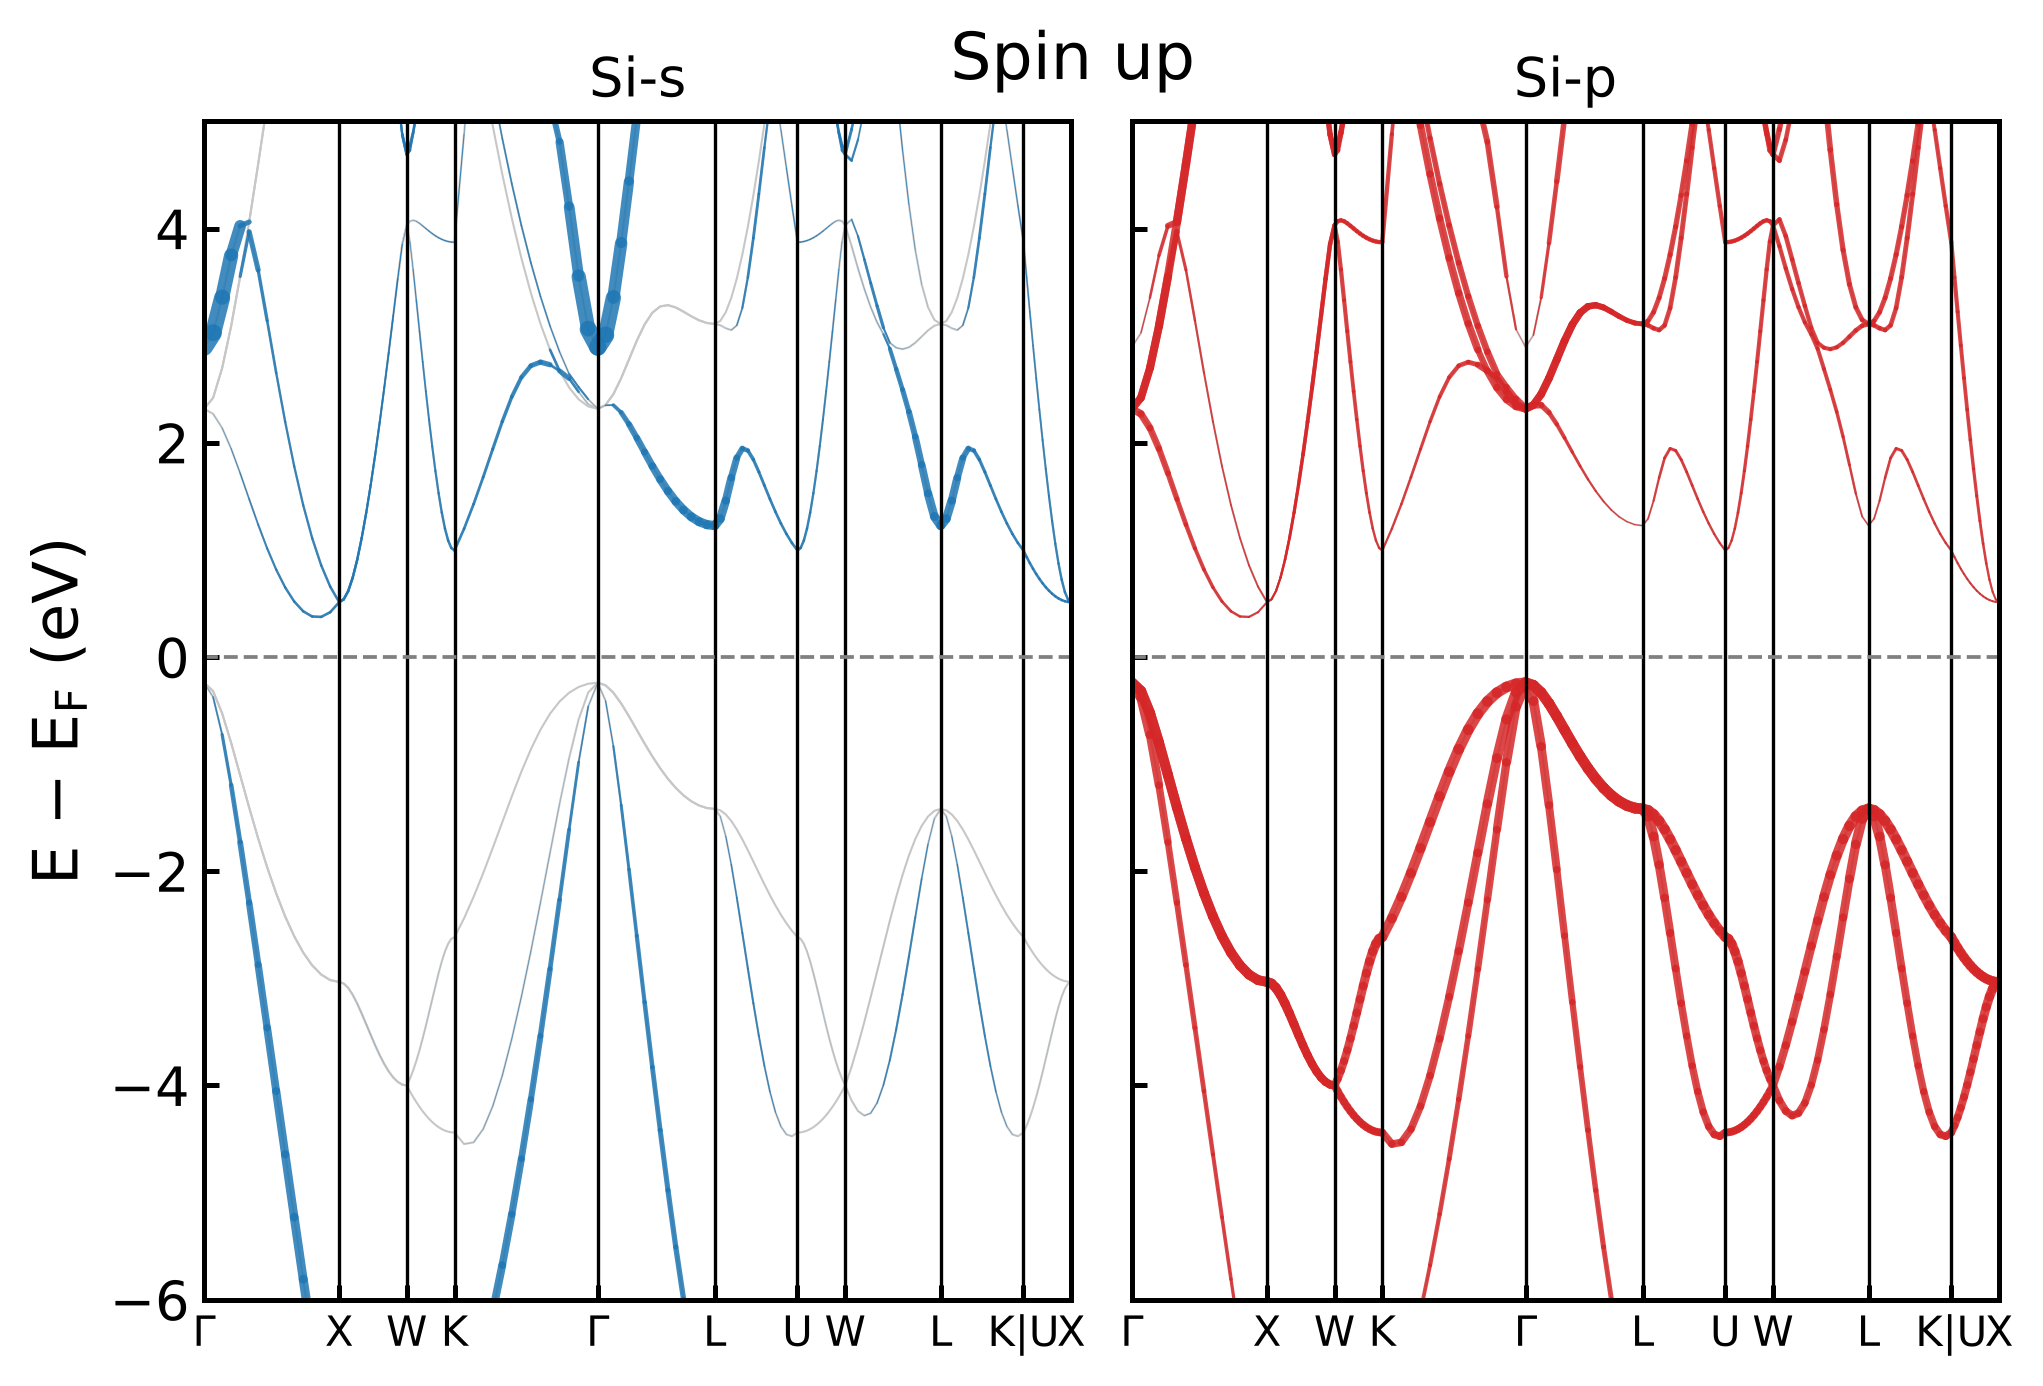
\includegraphics[width=0.49\linewidth]{fig/si_fat.png}\hfill
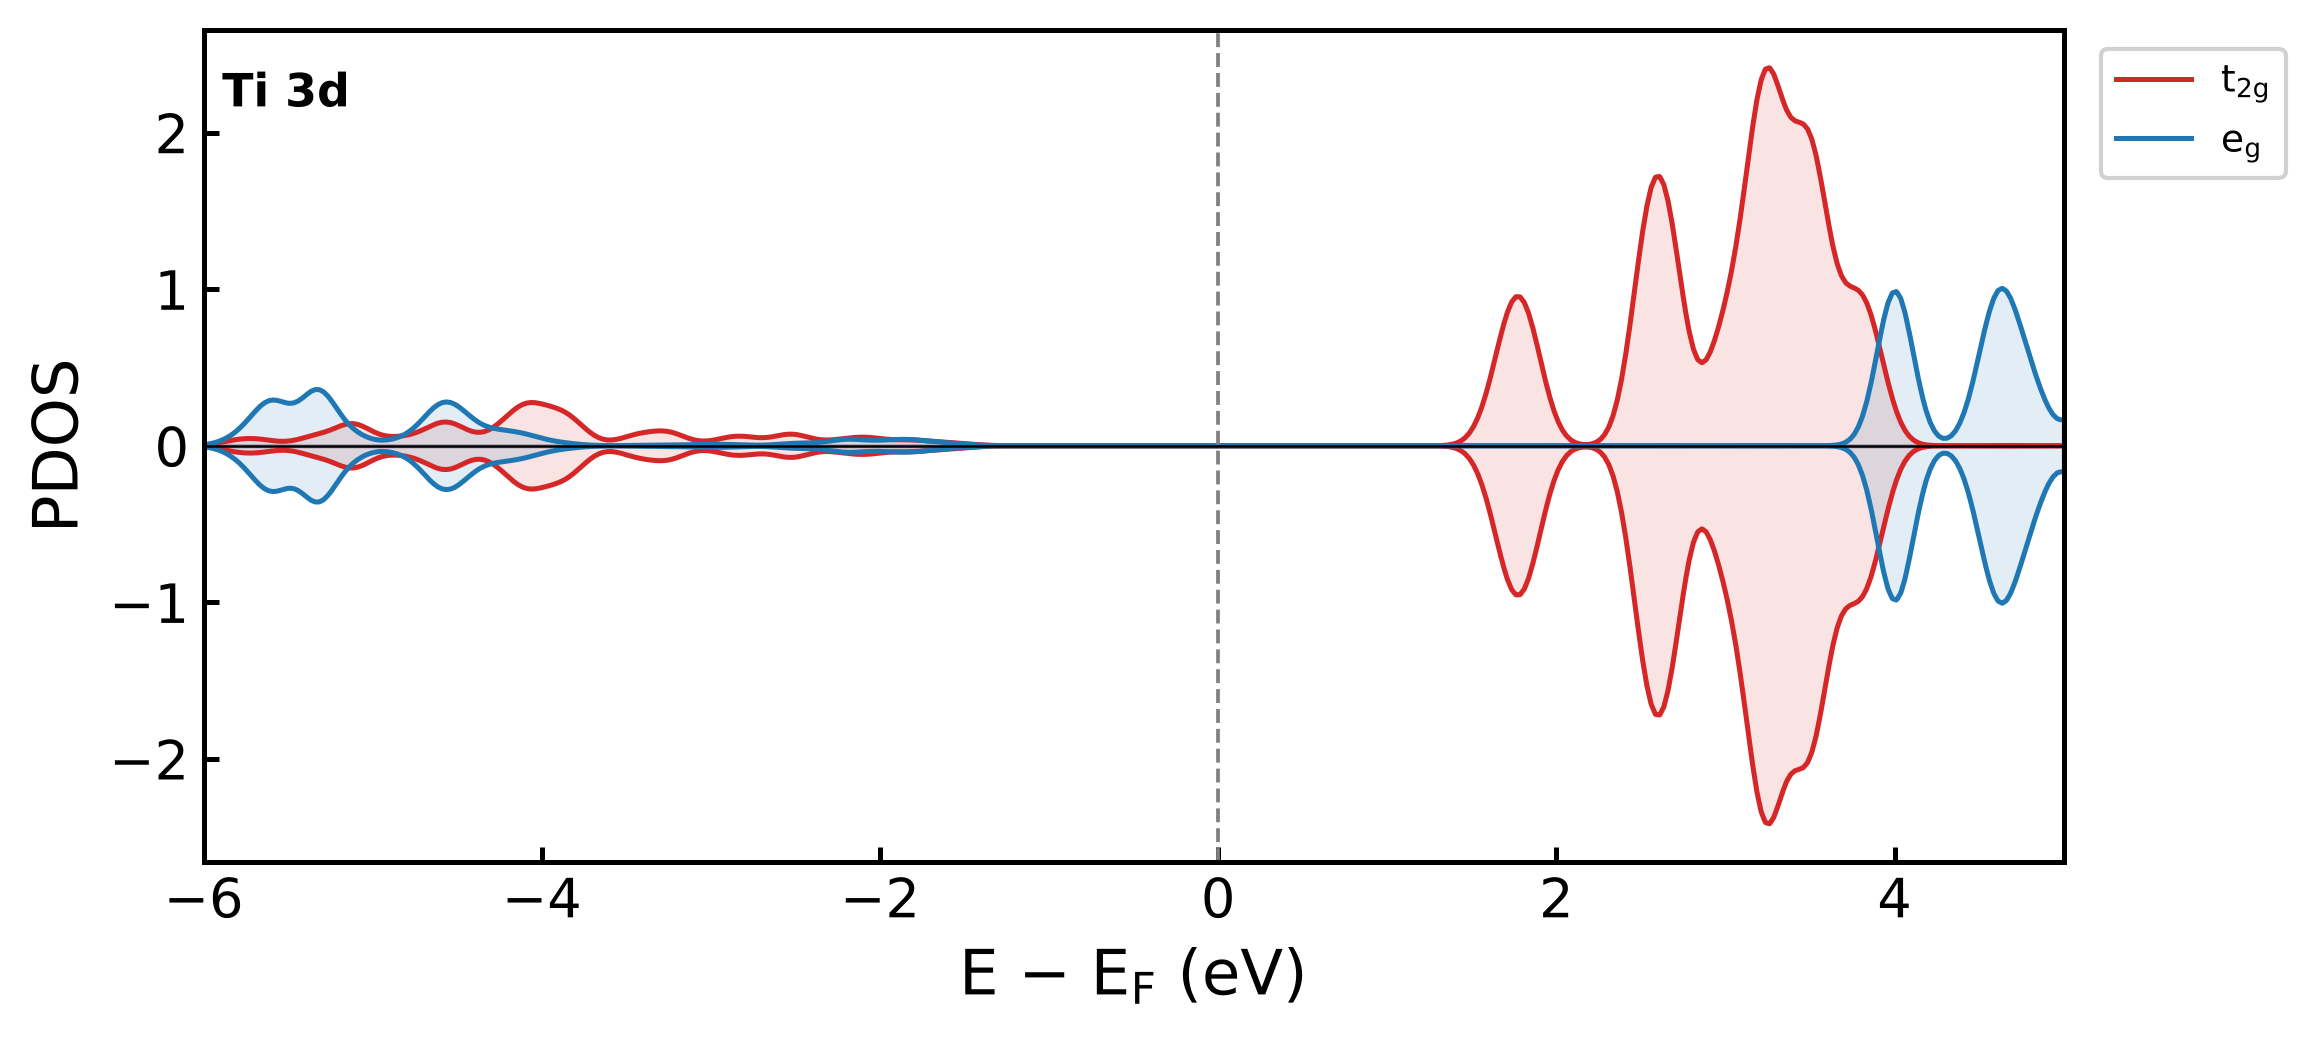
\includegraphics[width=0.49\linewidth]{fig/sto_t2g.png}
\caption{Left: projected bands of Si (VASP): $s$ character at the bottom of the valence band and $p$ character at its top. Right: Ti~3d PDOS of SrTiO$_3$ (SIESTA) split into $t_{2g}$ and $e_g$ by the octahedral crystal field.}\label{fig:valid}
\end{figure}

\section{Application: Fe-substituted MgH$_2$}\label{sec:app}
We illustrate the workflow on a $3\times3\times3$ rutile MgH$_2$ supercell (162 atoms, $a=b=13.519$\,\AA, $c=9.001$\,\AA) in which one Mg is replaced by Fe, computed with CASTEP (PBE, spin-polarised). \BMR\ reads $\eF^{\uparrow}=0.067501$\,Ha and $\eF^{\downarrow}=0.067499$\,Ha from the \code{.bands} file and finds a total gap of 1.394\,eV, indirect between M and R in both channels, with flat Fe-$d$ states inside the host gap around $\eF$ (Fig.~\ref{fig:mgh2}, original energy scale with the Fermi level marked). The defect analysis identifies a substitution at the Mg site with an octahedral FeH$_6$ unit whose Fe–H bonds (1.649–1.653\,\AA) are 15.4\% shorter than the Mg–H bonds of the bulk (1.952\,\AA); the H–Mg bonds of the hydrogens bound to Fe lengthen by 4.6\% on average. The FeH$_6$ octahedron is almost regular ($\langle\lambda\rangle=1.0004$, $\sigma^2=1.5$\,deg$^2$), in contrast with the distorted MgH$_6$ octahedra of the host ($\langle\lambda\rangle=1.0105$, $\sigma^2=37.1$\,deg$^2$). These results, together with the charge-density analysis and the thermodynamic quantities computed from the elemental references, are the basis of the companion study of transition-metal substitution in MgH$_2$ \cite{macedo2025tcc}.

\begin{figure}[t]\centering
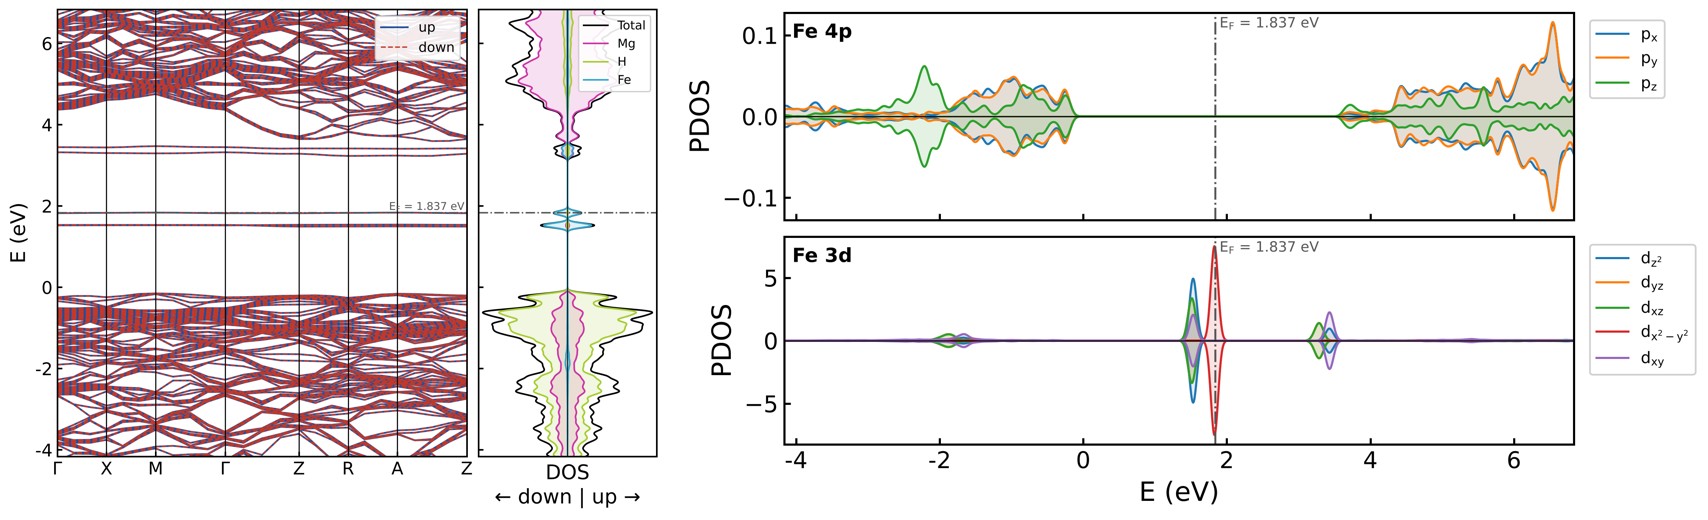
\includegraphics[width=\linewidth]{fig/fermi_python.png}
\caption{MgH$_2$:Fe (CASTEP) produced by the command line: band structure with total and element-projected DOS (left) and Fe~4p/3d $m$-resolved PDOS (right), in the original energy scale with the Fermi level ($\eF=1.837$\,eV) marked by a dash-dotted line.}\label{fig:mgh2}
\end{figure}

\begin{figure}[t]\centering
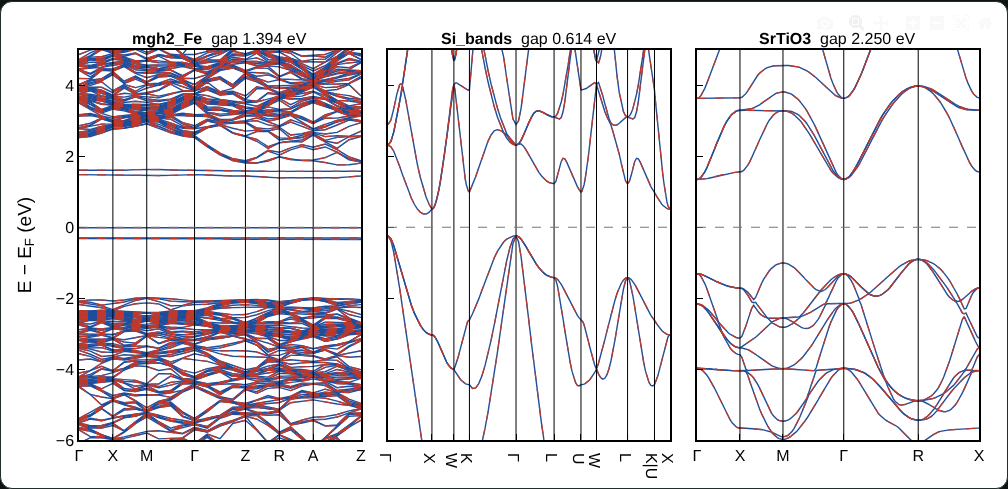
\includegraphics[width=\linewidth]{fig/comparison.png}
\caption{Comparison tab: band structures of calculations from three different codes (CASTEP MgH$_2$:Fe, VASP Si, SIESTA SrTiO$_3$) displayed side by side, each aligned at its own Fermi level.}\label{fig:cmp}
\end{figure}

\section{Limitations and outlook}
The band gap and band edges are evaluated on the $\bm{k}$-points of the computed path, so extrema located off the path are missed; densities of states computed from a band path are illustrative only and a dense mesh should be used for quantitative values. Orbital $m$ components and $t_{2g}/e_g$ sums refer to the Cartesian axes of the cell. Voronoi charges are geometrical estimates, and the browser version of the Bader partition omits the edge refinement applied by the command line. Thermodynamic quantities exclude zero-point and vibrational contributions, and comparisons of formation energies require identical functionals, cutoffs, pseudopotentials and Hubbard parameters. Planned extensions include work functions from planar-averaged electrostatic potentials, crystal orbital Hamilton populations from LOBSTER outputs, phonon dispersions, optical spectra and band unfolding.

\section{Conclusions}
\BMR\ unifies, in a single free program, analyses that usually require several tools, for the outputs of five widely used electronic-structure codes. Its common data model guarantees that every analysis behaves identically regardless of the code, its three front-ends serve interactive exploration, offline desktop use and automated cluster workflows with the same results, and its emphasis on preserving the Fermi energy, exporting plain data and tracking citations supports reproducible and properly credited research. The program, its tutorial in six languages and validation examples are freely available.

\section*{Acknowledgements}
The author thanks Benedet, R. O., without whom this work would never have happened. The author acknowledges the Conselho Nacional de Desenvolvimento Científico e Tecnológico (CNPq, Brazil) for the master's scholarship, the Programa de Pós-Graduação em Física Aplicada of UNILA, and Prof. J. R. C. Salgado and Prof. R. S. da Lapa for supervision. The developers of CASTEP, VASP, SIESTA, Quantum ESPRESSO and ORCA, and of the test suites of pymatgen, sisl and cclib, are gratefully acknowledged for the reference outputs used in validation.

\section*{Code and data availability}
Source code, issue tracker and releases: \url{https://github.com/brunohdmacedo/brumare}. Web application and tutorial (six languages): \url{https://brunohdmacedo.tech/brumare/}. The Python package is distributed through PyPI as \code{brumare}. All validation inputs are publicly available in the cited test suites; the MgH$_2$:Fe outputs are available from the author upon reasonable request.

\section*{CRediT authorship contribution statement}
\textbf{Bruno Henrique Dourado Macedo:} Conceptualization, Methodology, Software, Validation, Formal analysis, Investigation, Data curation, Visualization, Writing – original draft, Writing – review \& editing.

\section*{Declaration of competing interest}
The author declares no known competing financial interests or personal relationships that could have appeared to influence the work reported in this paper.

\appendix
\section{Implementation map}\label{app:map}
Table~\ref{tab:map} relates each method to the functions that implement it in the command-line program (\code{brumare.py}) and in the web/desktop application (\code{index.html}).

\begin{small}
\begin{longtable}{@{}p{0.30\linewidth}p{0.33\linewidth}p{0.31\linewidth}@{}}
\caption{Where each method is implemented.}\label{tab:map}\\\toprule
Method & Python (\code{brumare.py}) & JavaScript (\code{index.html}) \\\midrule\endfirsthead
\toprule Method & Python & JavaScript \\\midrule\endhead
CASTEP readers & \code{read\_bands}, \code{read\_pdos\_bin}, \code{read\_castep\_extra}, \code{read\_castep\_struct}, \code{read\_cell\_struct} & \code{parseBands}, \code{parsePdosBin}, \code{parseCastep}, \code{parseCellStruct} \\
$\bm{k}$-point alignment & \code{align\_k} & \code{alignK} \\
VASP reader & \code{read\_vasprun}, \code{load\_vasp} & \code{parseVasprun} \\
SIESTA readers & \code{read\_siesta\_bands}, \code{read\_siesta\_pdos}, \code{read\_siesta\_rho} & \code{parseSiestaBands}, \code{parseSiestaPDOS}, \code{parseSiestaRHO} \\
QE and ORCA readers & \code{read\_qe\_xml}, \code{read\_orca} & \code{parseQE}, \code{parseORCA}, \code{orcaToSeed} \\
Code detection, virtual registry & \code{detect\_code}, \code{prepare\_inputs} & \code{classify} \\
Band path and labels & \code{kpath} & \code{kPath} \\
Energy reference, Fermi line & \code{linha\_ef} (original-energy axis) & \code{eWin}, \code{efLines} \\
DOS and PDOS & \code{gaussian\_dos}, \code{build\_orbitals}, \code{make\_groups} & \code{dosCurve}, \code{getDos}, \code{curveDos}, \code{buildOrbitals}, \code{groupsFor} \\
Band edges, gaps & \code{band\_edges} & \code{bandEdges} \\
Effective masses & \code{massas\_efetivas} & analysis tab \\
Band-gap correction & \code{correcao\_gap}, \code{aplicar\_tesoura} & \code{corrigirGap}, \code{gapCorrHTML} \\
Brillouin zone and k-path & \code{bz\_compute}, \code{bz\_classify}, \code{bz\_path}, \code{bz\_textos} & \code{bzCompute}, \code{bzClassify}, \code{bzPath}, \code{bzTextos} \\
Defect analysis & \code{analyze\_defect}, \code{defect\_report} & \code{analyzeDefect}, \code{guessDefect}, \code{renderDefect} \\
Thermodynamics & \code{thermo} & defect tab \\
Densities and planes & \code{read\_density}, \code{read\_chgcar}, \code{planes\_report}, \code{density\_report} & \code{parseDenFmt}, \code{parseCHGCAR}, \code{parseCube}, \code{planeFromHKL}, \code{renderPlanes} \\
Voronoi and Bader & \code{voronoi\_report}, \code{bader\_ongrid}, \code{\_bader\_refinar} & \code{voronoiPartition}, \code{baderPartition} \\
Density difference & \code{diff\_report} & density-difference tab \\
VESTA export & \code{vesta\_export} & VESTA package export \\
Comparison & \code{compare\_report} & comparison tab \\
Citation tracking & \code{write\_citation} & \code{bibUsado} \\\bottomrule
\end{longtable}
\end{small}

\bibliographystyle{unsrtnat}
\bibliography{artigo}
\end{document}
